
% These macros come from my dissertation.
\newcommand{\cedge}[1]{\stackrel{#1}{\longleftarrow}}
\newcommand{\cred}[3]{\mathit{#1} \cedge{#3} \mathit{#2}}
\newcommand{\datalog}{\text{Datalog}}
\newcommand\T{\rule{0pt}{2.1ex}}

\startslide{Outline}
% The outline follows the structure of my dissertation. Why not?
\begin{cenumerate}
\item Introduction
\item Review of Trust Management
\item SpartanRPC/Sprocket
\item DScalaness/DnesT
\item Scalaness/nesT
\item Evaluation
\item Conclusion
\end{cenumerate}
\stopslide

%%%%%

\startslide{Introduction}
This is wonderful!
\stopslide

%%%%%

\startslide{Outline}
\begin{cenumerate}
\item Introduction
\item \cemph{Review of Trust Management}
\item SpartanRPC/Sprocket
\item DScalaness/DnesT
\item Scalaness/nesT
\item Evaluation
\item Conclusion
\end{cenumerate}
\stopslide

%%%%%

\startslide{Structure of Trust Management Systems}
\begin{tabular}{cc}
\scalebox{1.75}{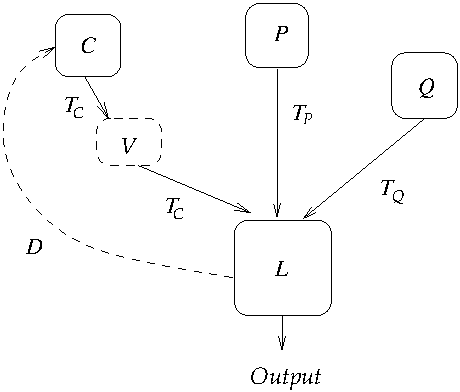
\includegraphics{Figures/tmstruct.pdf}}
& 
\hspace{-10mm}
$
\begin{array}[b]{rcl}
P &:& \text{Policy}\\
C &:& \text{Certificates}\\
Q &:& \text{Authorization Query}\\
V &:& \text{Certificate Validation}\\
L &:& \text{Authorization Mechanism}\\
T_P &:& \text{Policy Compilation}\\
T_C &:& \text{Credential Encoding}\\
T_Q &:& \text{Query Compilation}\\
D &:& \text{Certificate Discovery}\\
\end{array}
$
\end{tabular}
\stopslide

%%%%%

\startslide{$RT_0$ Credential Forms}
Simplest member of the $RT$ family\footnote{\textit{Design of a Role-based Trust-management
    Framework}, Mitchell \& Winsborough, 2002}.
\begin{cenumerate}
\item $\cred{A.r}{E}{}$ 
\item $\cred{A.r}{B.s}{}$ 
\item $\cred{A.r}{B.s.t}{}$ 
\item $\cred{A.r}{f_1 \cap \cdots \cap f_n}{}$
\end{cenumerate}
\stopslide

%%%%%

\startslide{$RT_0$ Foundation}
\begin{cenumerate}
\item $\cred{A.r}{E}{}$

$\textit{isMember}(E, A, r).$

\item $\cred{A.r}{B.s}{}$

$\textit{isMember}(\textit{?x}, A, r) \leftarrow
 \textit{isMember}(\textit{?x}, B, s).$

\item $\cred{A.r}{B.s.t}{}$

$\textit{isMember}(\textit{?x}, A, r) \leftarrow
 \textit{isMember}(\textit{?y}, B, s),
 \textit{isMember}(\textit{?x}, \textit{?y}, t).$

\item $\cred{A.r}{B_1.s_1 \cap \cdots \cap B_n.s_n}{}$

$\textit{isMember}(\textit{?x}, A, r) \leftarrow
 \textit{isMember}(\textit{?x}, B_1, s_1), \ldots,
 \textit{isMember}(\textit{?x}, B_n, s_n).$
\end{cenumerate}
\stopslide

%%%%%

\startslide{How it Works}
\begin{cenumerate}
\item Alice $A$ has policy $P$ protecting some resource.
\item Bob $B$ submits certificates $\mathcal{C}$ to $A$ with access request signed by $B$.
\item $A$ checks validity on each $c \in \mathcal{C}$ and collects valid credentials in set $C$.
\item $A$ converts $P\,' = P \cup C$ to \datalog\ rules $\mathcal{D}$.
\item Access is granted if $B$ is a member of some \textit{governing role} according to
  $\mathcal{D}$.
\end{cenumerate}
\stopslide

%%%%%

\startslide{Example}
\begin{citemize}
\item \texttt{Alice.records} $\leftarrow$ \texttt{Bob}
\item \texttt{Alice.records} $\leftarrow$ \texttt{Bob.alice\_delegates}
\item \texttt{Bob.team} $\leftarrow$ \texttt{Carol}
\item \texttt{Bob.team} $\leftarrow$ \texttt{Bob.team.support}
\item \texttt{Bob.alice\_delegates} $\leftarrow$
  \texttt{Hospital.medical\_staff} $\cap$ \texttt{Bob.team}
\item \texttt{Carol.support} $\leftarrow$ \texttt{Dave}
\item \texttt{Hospital.medical\_staff} $\leftarrow$ \texttt{Dave}
\end{citemize}
\stopslide

%%%%%

\startslide{Why $RT_0$?}
\begin{citemize}
\item \cemph{Formal foundation} based on \datalog.
\item \cemph{Expressive} enough to write interesting policies.
\item \cemph{Simple} enough to implement in limited space/time.
\item \cemph{Understandable} enough to avoid configuration errors.
\end{citemize}
\stopslide

%%%%%

\startslide{Outline}
\begin{cenumerate}
\item Introduction
\item Review of Trust Management
\item \cemph{SpartanRPC/Sprocket}
\item DScalaness/DnesT
\item Scalaness/nesT
\item Evaluation
\item Conclusion
\end{cenumerate}
\stopslide

%%%%%

\startslide{Security Protocol}
\centerline{\scalebox{0.85}{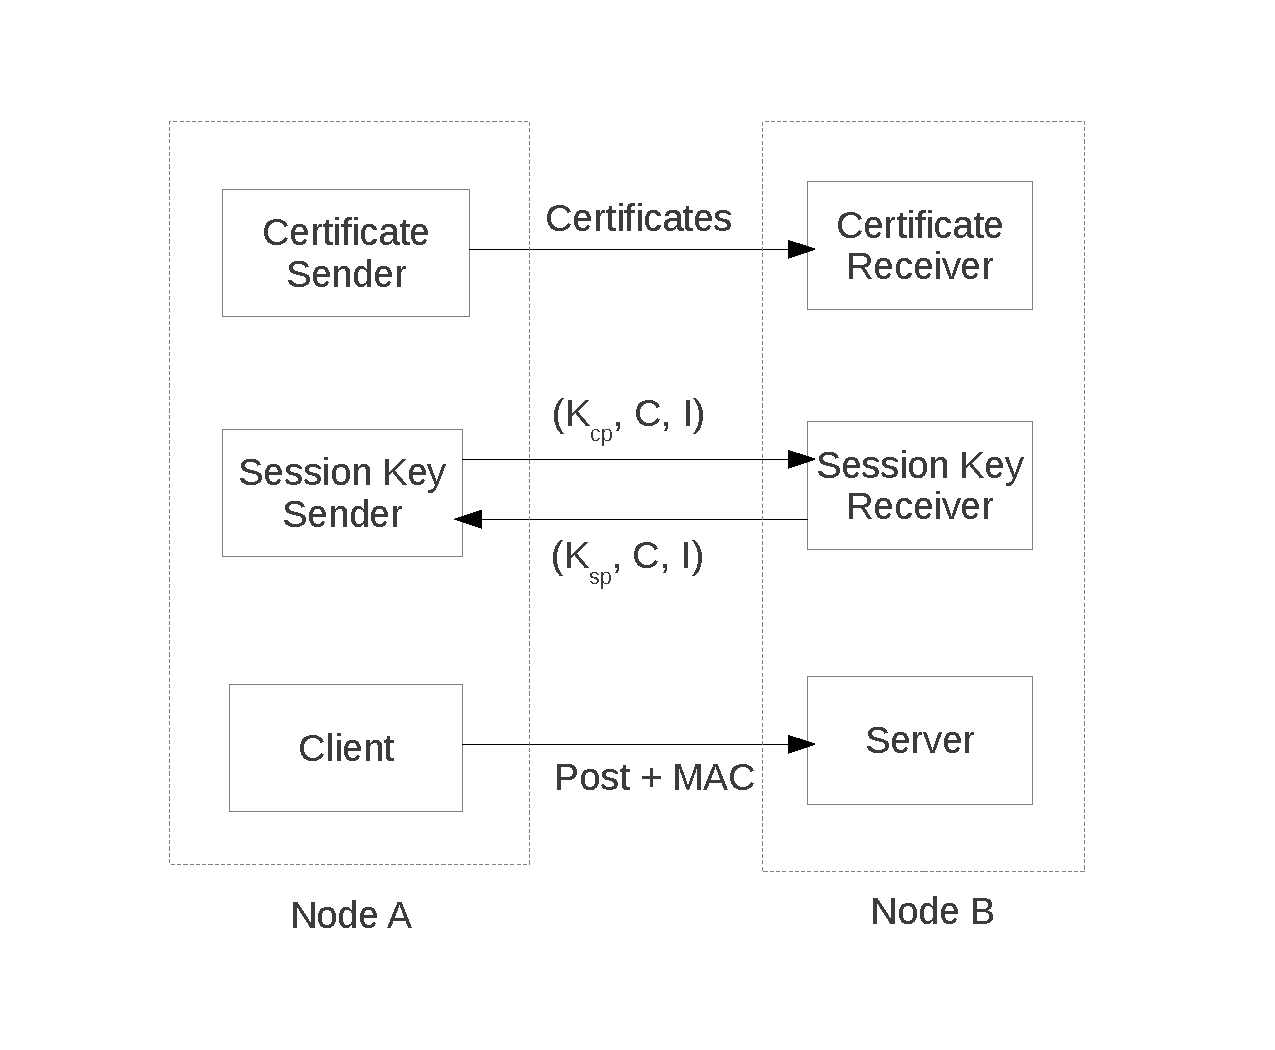
\includegraphics{Figures/SprocketRT-Protocol.pdf}}}
\stopslide

%%%%%

\startslide{Certificate Receiver}
\centerline{\scalebox{0.55}{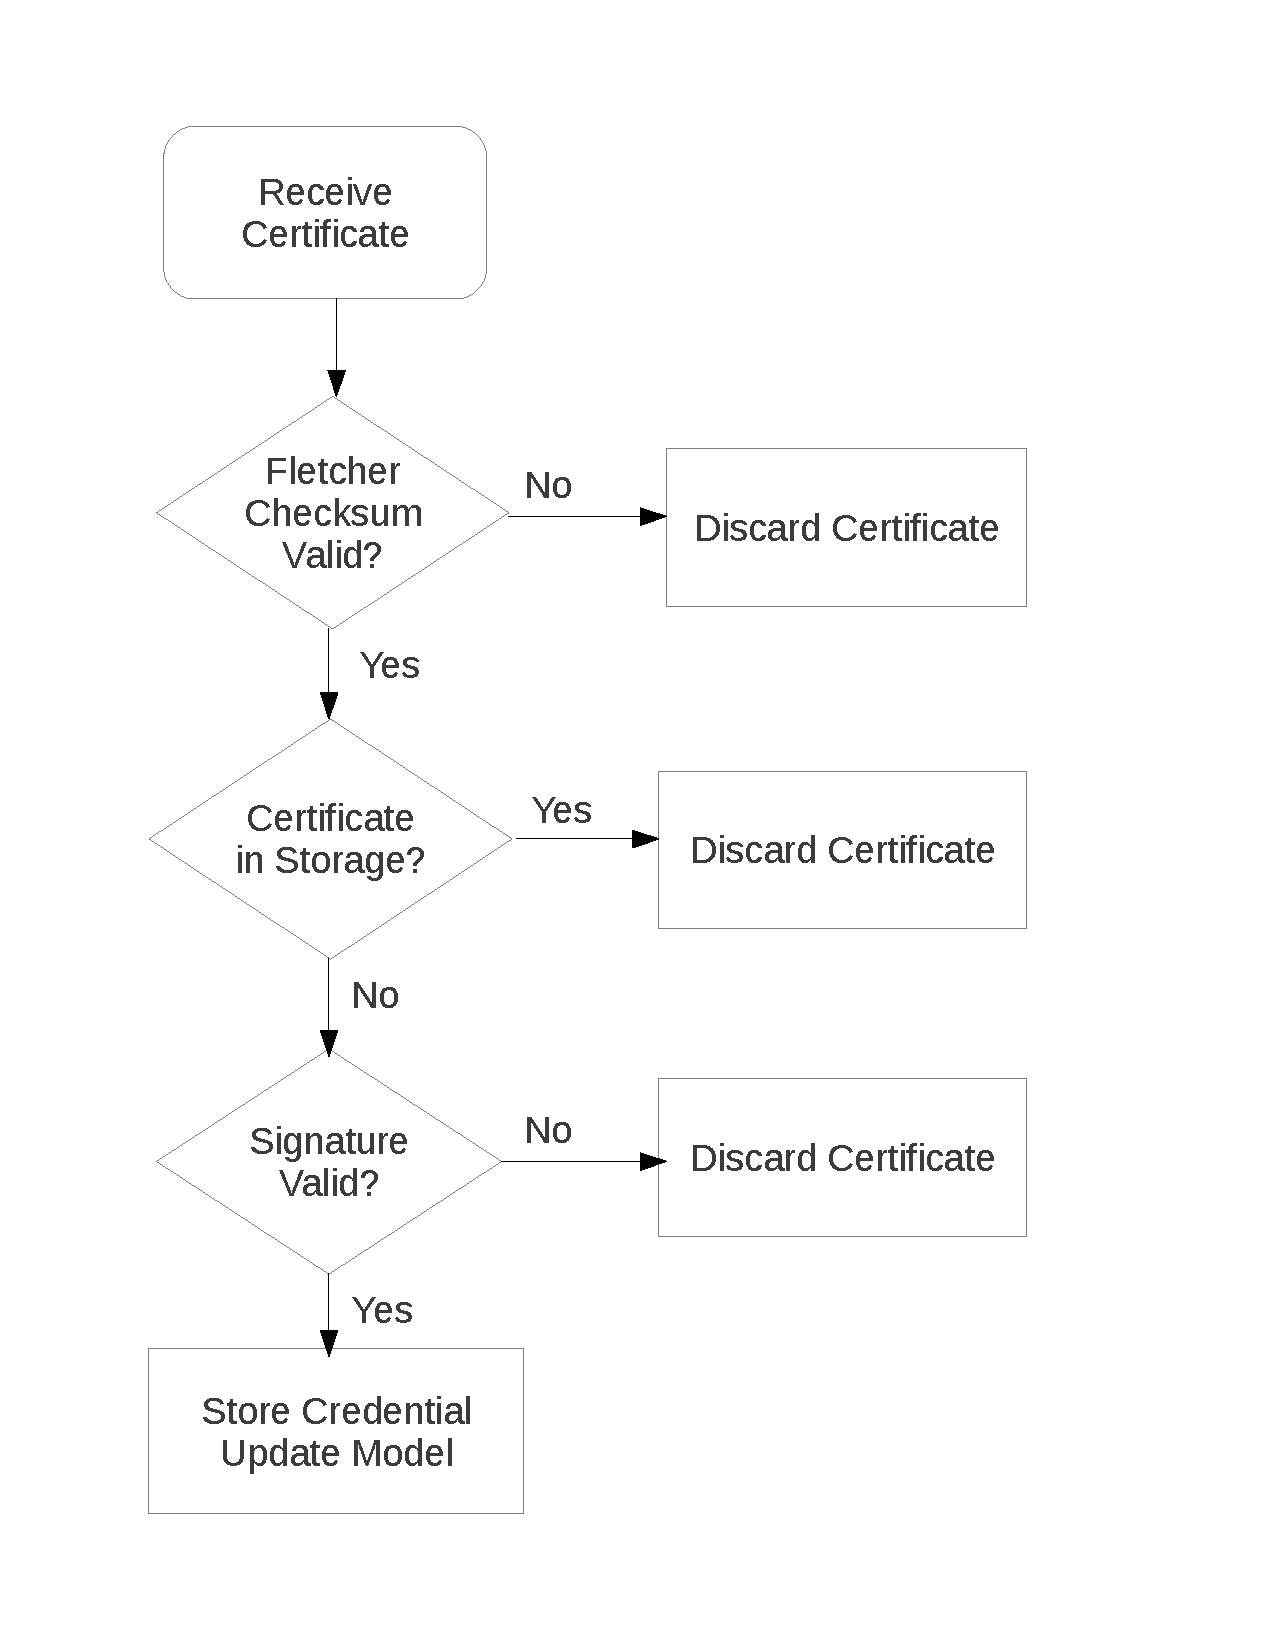
\includegraphics{Figures/Certificate-Receiver-Flowchart.pdf}}}
\stopslide

%%%%%

\startslide{Post Duty}
\centerline{\scalebox{0.70}{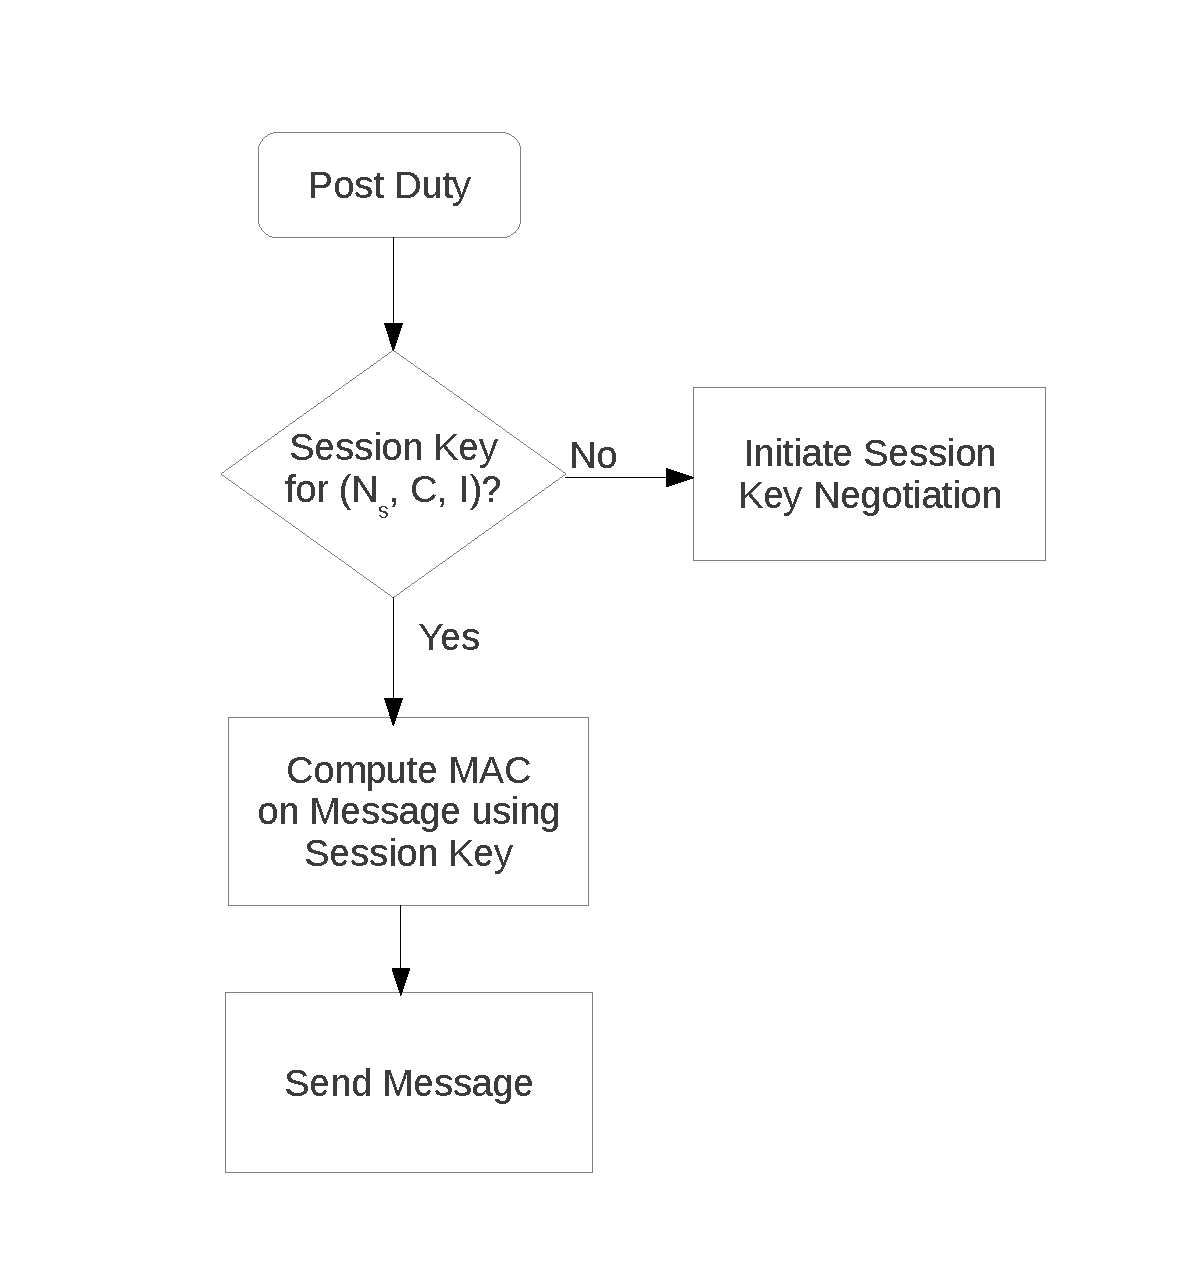
\includegraphics{Figures/Post-Duty-Flowchart.pdf}}}
\stopslide

%%%%%

\startslide{Post Format}
\centerline{\scalebox{1.0}{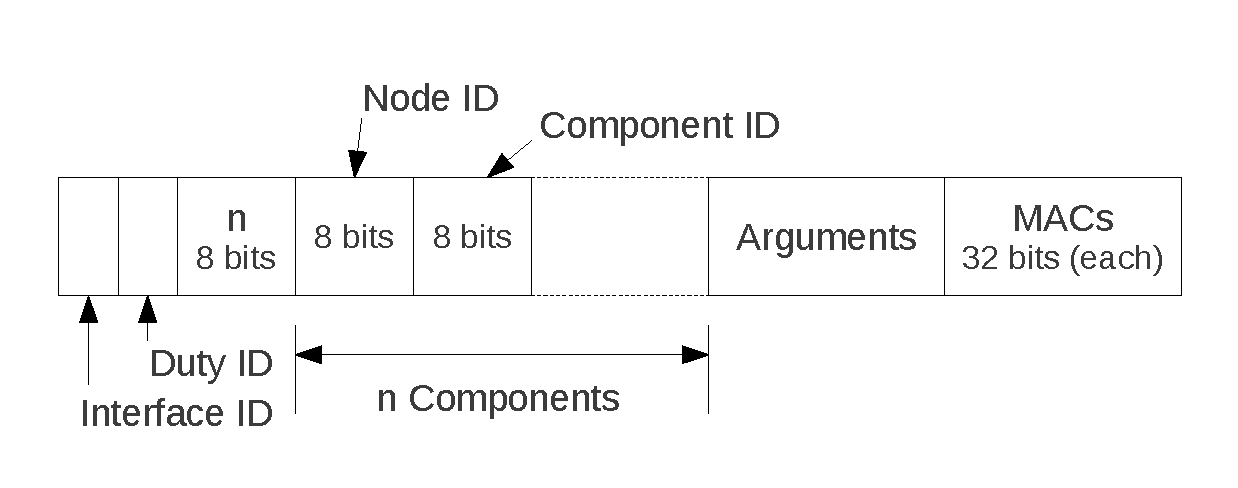
\includegraphics{Figures/Post-Format.pdf}}}
\stopslide

%%%%%

\startslide{Receive Duty}
\centerline{\scalebox{0.70}{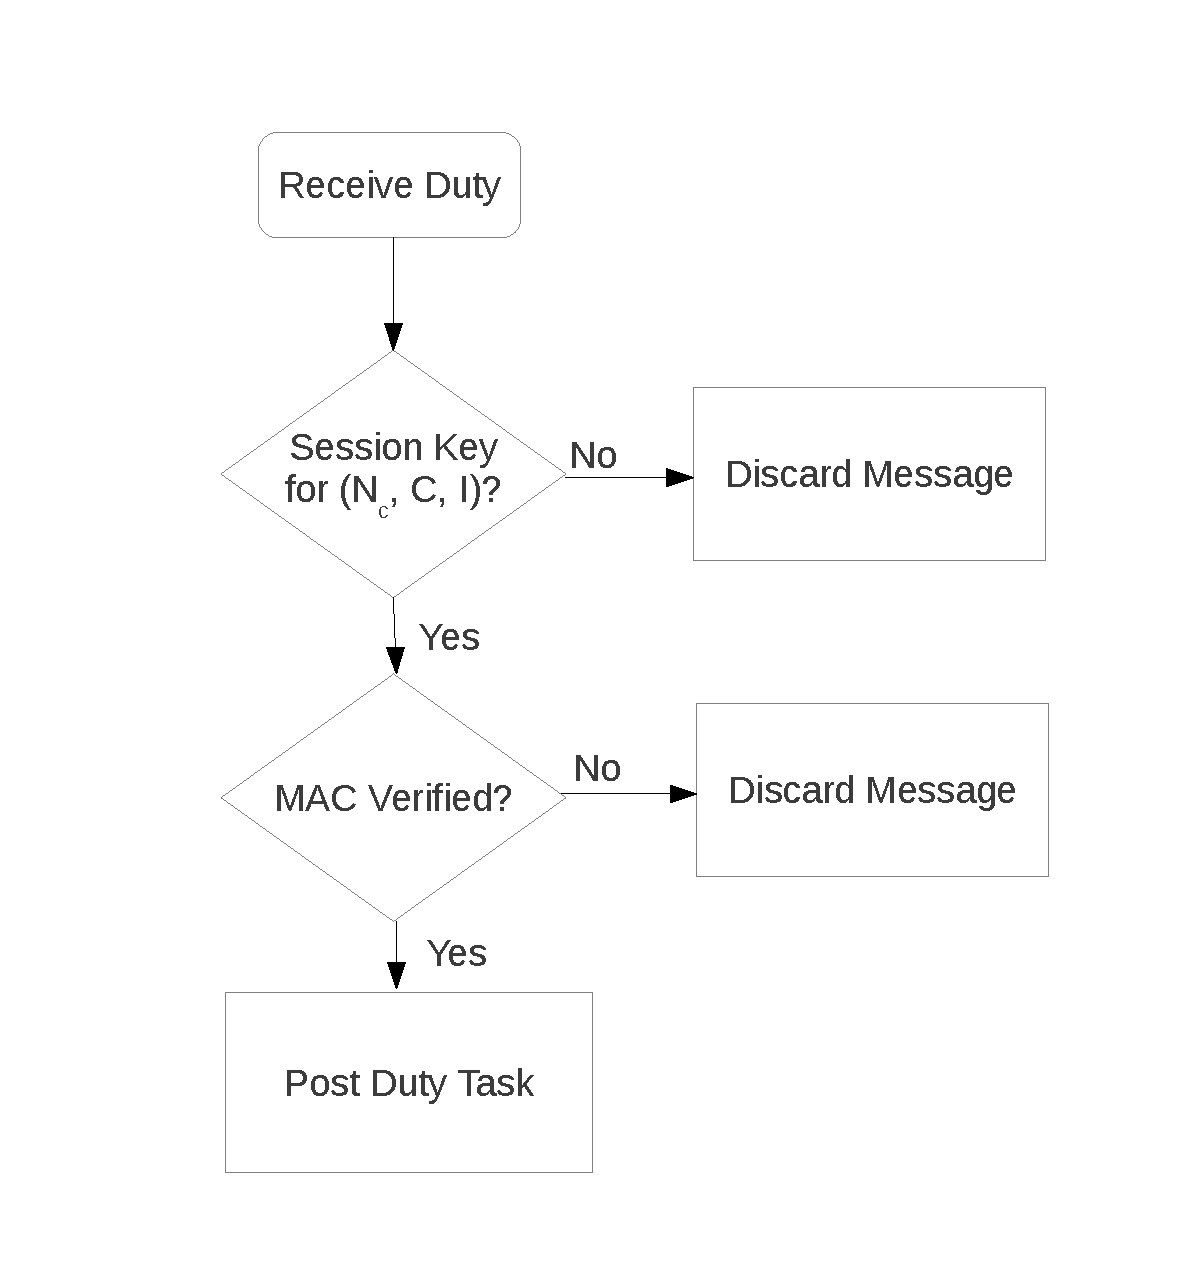
\includegraphics{Figures/Receive-Duty-Flowchart.pdf}}}
\stopslide

%%%%%

\startslide{Session Key Sender}
\centerline{\scalebox{0.85}{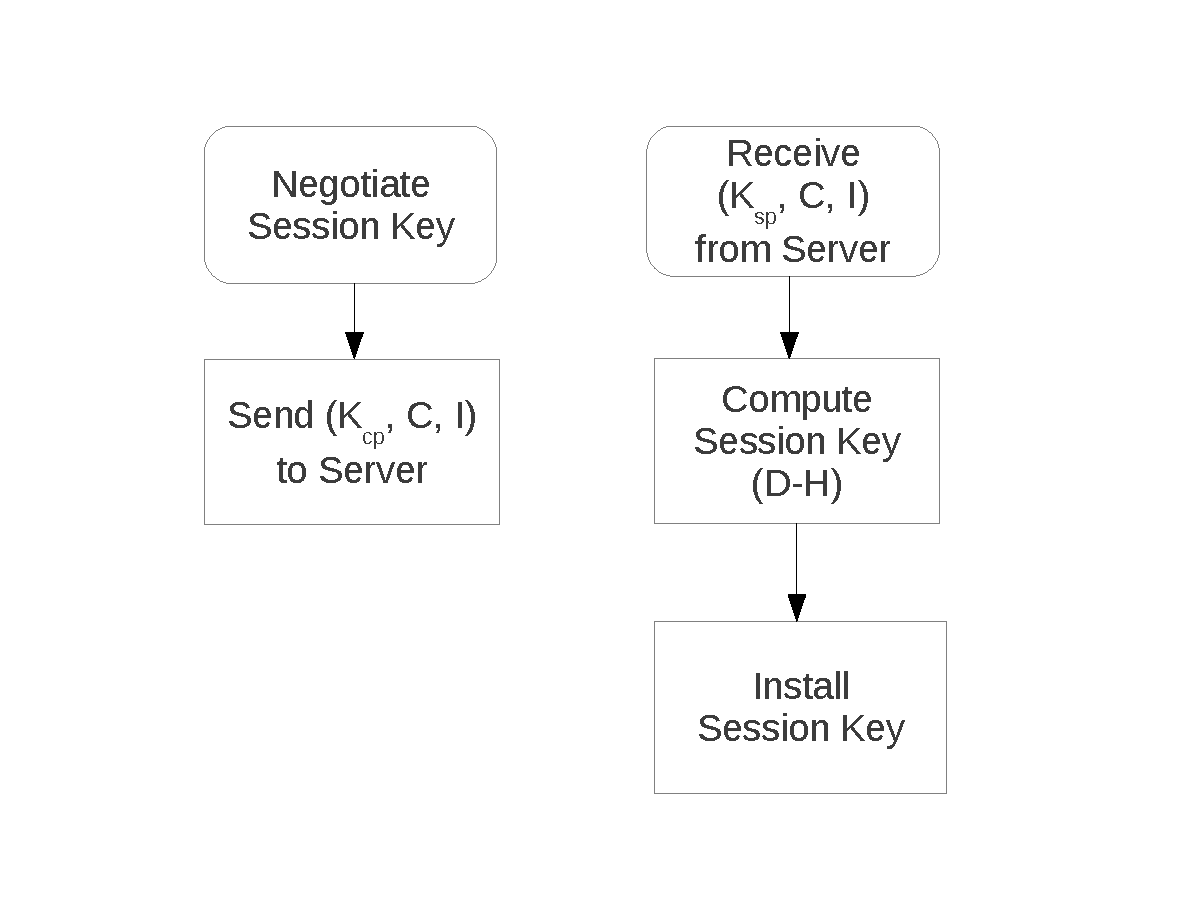
\includegraphics{Figures/SessionKey-Sender-Flowchart.pdf}}}
\stopslide

%%%%%

\startslide{Session Key Receiver}
\centerline{\scalebox{0.60}{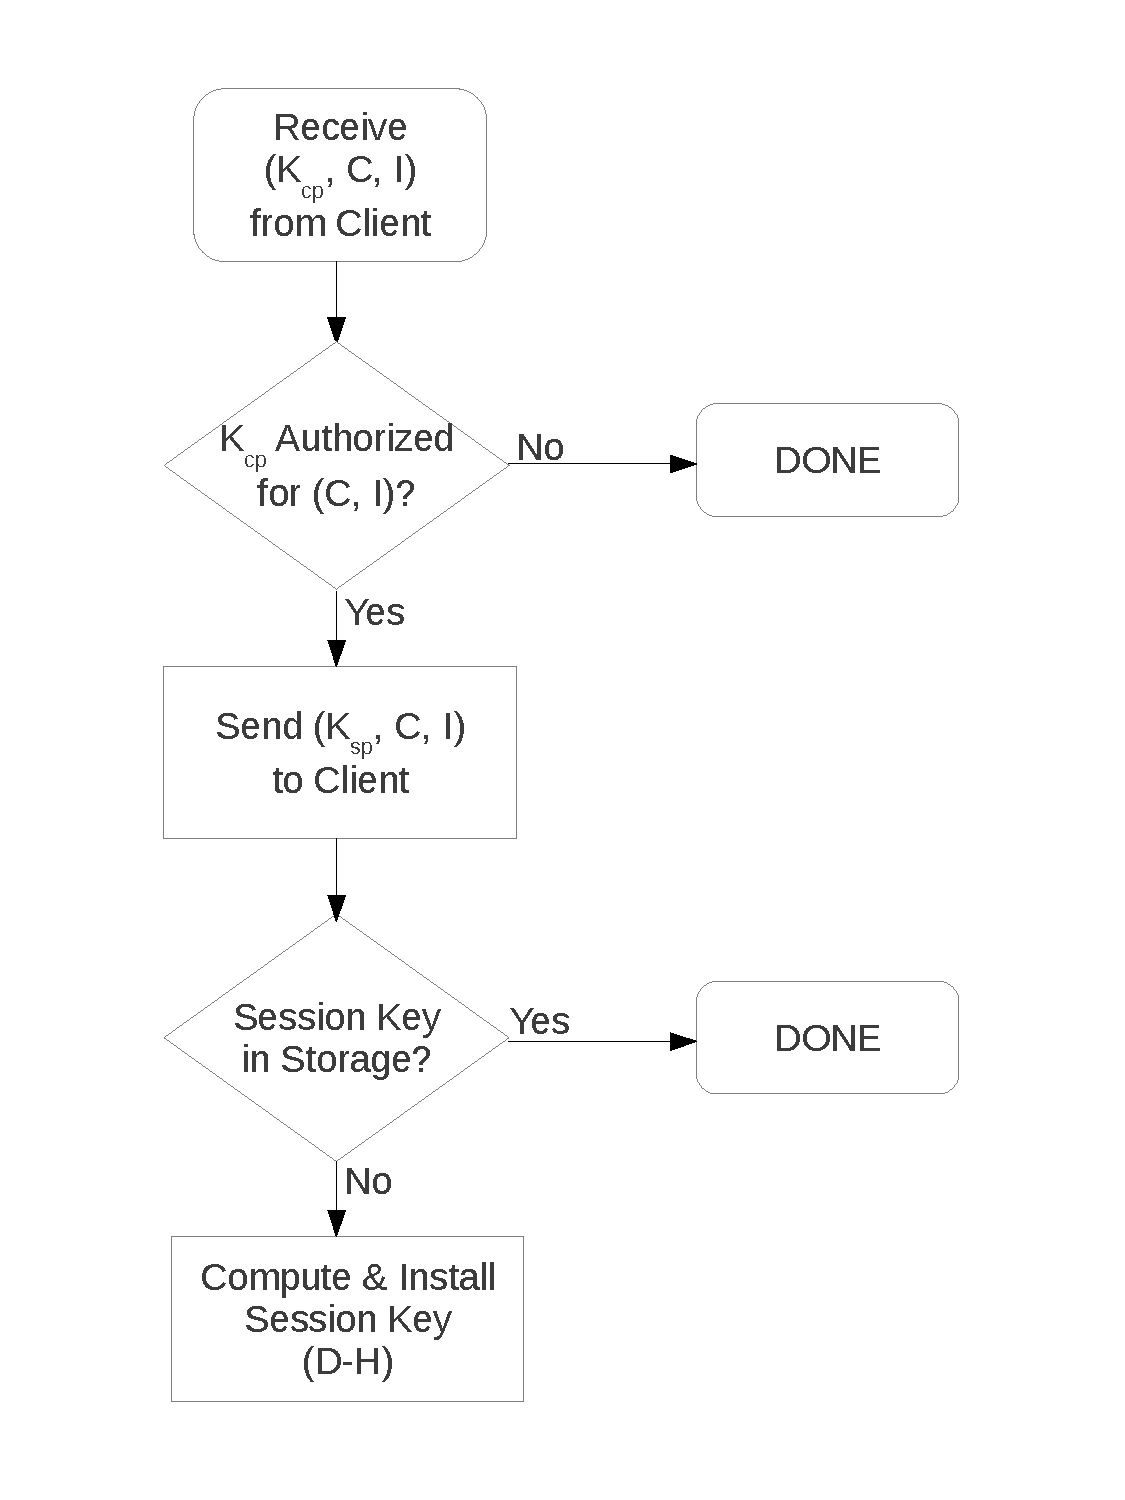
\includegraphics{Figures/SessionKey-Receiver-Flowchart.pdf}}}
\stopslide

%%%%%

\startslide{Outline}
\begin{cenumerate}
\item Introduction
\item Review of Trust Management
\item SpartanRPC/Sprocket
\item \cemph{DScalaness/DnesT}
\item Scalaness/nesT
\item Evaluation
\item Conclusion
\end{cenumerate}
\stopslide

%%%%%

\startslide{Outline}
\begin{cenumerate}
\item Introduction
\item Review of Trust Management
\item SpartanRPC/Sprocket
\item DScalaness/DnesT
\item \cemph{Scalaness/nesT}
\item Evaluation
\item Conclusion
\end{cenumerate}
\stopslide

%%%%%

\startslide{Outline}
\begin{cenumerate}
\item Introduction
\item Review of Trust Management
\item SpartanRPC/Sprocket
\item DScalaness/DnesT
\item Scalaness/nesT
\item \cemph{Evaluation}
\item Conclusion
\end{cenumerate}
\stopslide

%%%%%

\startslide{Sprocket RAM Overhead}
\centering
  \begin{tabular}{|l|r|r|r|} \hline
    \textit{Storage Area} \T & \textit{\# Items} & \textit{Bytes/Item} & \textit{Total Bytes} \\
    \hline \hline

    Session Keys ($n_k$) \T & 10 & 22 & 220 \\ \hline 
    Public Keys ($n_p$)  \T & 12 & 40 & 480 \\ \hline
    Credentials ($n_c$ ) \T & 12 & 16 & 192 \\ \hline
    Model ($n_m$)        \T & 16 &  6 &  96 \\ \hline \hline
    \textbf{Total} \T & \multicolumn{3}{r|}{ \textbf{988} } \\ \hline
  \end{tabular}
\stopslide

%%%%%

\startslide{Memory Consumption of Minimal Test Programs}
\centering
  \begin{tabular}{|l|r|r|} \hline
    \textit{Test Program} \T & \textit{RAM Bytes} & \textit{ROM Bytes} \\
    \hline \hline

    Baseline Client    \T &  349 & 10982 \\ \hline 
    Baseline Server    \T &  283 & 10490 \\ \hline
    SpartanRPC Client  \T & 2222 & 23108 \\ \hline
    SpartanRPC Server  \T & 2126 & 23394 \\ \hline
    Directed Diffusion \T & 3105 & 27826 \\ \hline
  \end{tabular}
\stopslide

%%%%%

\startslide{Maximum Message Transfer Rate}
\centering
  \begin{tabular}{|l|r|r|} \hline
    \textit{Test} \T & \textit{messages/s} & \textit{\% Reduction} \\
    \hline \hline

    Baseline \T & 128 &   -- \\ \hline 
    Duties   \T & 119 &  7.0 \\ \hline
    MAC      \T &  87 & 32.0 \\ \hline
  \end{tabular}
\stopslide

%%%%%

\startslide{Processing Time for Transient Operations}
\centering
  \begin{tabular}{|l|r|} \hline
    \textit{Operation} \T & \textit{Time} \\ \hline \hline

    Certificate Verification     \T &  82s \\ \hline 
    Minimum Model Construction   \T & 370$\mu$s \\ \hline
    Session Key Negotiation      \T &  80s\\ \hline
  \end{tabular}
\stopslide

%%%%%

\startslide{Transient Time in Single Hop Directed Diffusion}
\centering
  \begin{tabular}{|l|r|r|r|} \hline
    \textit{\# neighbors} \T & \textit{1 Cert }
                             & \textit{2 Certs}
                             & \textit{3 Certs} \\ \hline \hline

    1 \T &  4m03s & 5m27s &  6m52s \\ \hline
    2 \T &  5m16s & 6m50s &  8m24s \\ \hline
    3 \T &  6m32s & 7m57s &  9m30s \\ \hline
    4 \T &  7m50s & 9m22s & 10m51s \\ \hline
  \end{tabular}
\stopslide

%%%%%

\startslide{Transient Time in Multi Hop Directed Diffusion}
\centering
  \begin{tabular}{|l|r|r|r|} \hline
    \textit{Run} \T & \textit{1 hop }
                    & \textit{2 hops}
                    & \textit{3 hops} \\ \hline \hline

                   1 \T &  4m05s & 7m24s & 9m10s \\ \hline
                   2 \T &  3m12s & 5m12s & 6m30s \\ \hline
                   3 \T &  3m57s & 7m37s & 9m15s \\ \hline
                   4 \T &  4m09s & 7m15s & 8m49s \\ \hline
    \textit{Average} \T &  3m51s & 6m52s & 8m23s \\ \hline
  \end{tabular}
\stopslide

%%%%%

\startslide{Conclusion}
Life is wonderful!
\stopslide